\chapter{Empirical Study}
\label{chapter3}

*Whole Chapter is Under construction* 

% @TODO Define a W-Structure.

The main objective of the empirical study if twofold. Firstly to correlate the iterations needed to collapse the contour tree in the merge phase of the algorithm with its w-diameter. Secondly to demonstrate that w-structures are found in real world data and do appear more abundantly as the size of datasets increases. As a result of this study we will be able to shed light on the practical obstacles that the w-structures pose. We are hopeful that this is the first step to overcoming them.

In addition to the main objectives there are some additional topics, related to the empirical study, that will be discussed:

\begin{itemize}
    \item Description the implementation of all used algorithms.
    \item Demonstration of the running time of the implementations of the algorithms.
    \item Determining the smallest 2-dimensional grid dataset that exhibits a w-structure.
    \item Discussion on whether it is possible to determine the w-diameter of a datasets without computing it's contour tree beforehand.
    \item Discussion on the kinds of structures in raw data that produce w-structures in the contour trees.
\end{itemize}


\section{Algorithms Implemented}

For the dissertation I implemented the one following algorithms - contour tree, 2xBFS, DP.

The first algorithm that had to be implemented was for computing the Contour Tree. For simplicity I implemented a version that takes as input a rectangular 2-dimensional mesh. I used the pseudocode provided in this paper [] and implemented it in C++. To test the correctness of the code I compared it against the code that was used for [].

After this I implemented three algorithm for w-detection. The first one is the most basic exhaustive approach where we find the w-length of all paths in the tree. It has quadratic running time. The second one is the 2xBFS algorithm and lastly the DP algorithm. They were implemented in C++. You can find the code in the appendix.

Another algorithm I implemented is one that generates all possible $n \times m$ 2-d grids. The objective here is to find the minimum one that produces a w-structure.

Lastly I implemented the algorithm in [] that computes extended persistence. I did this to verify the claims that I will make in the next chapter about the pairing of the global minimum and maximum.

All of the implementation are serial and not attempt has been made to parallelise them. There was simply no point in that as it is not the main objective of this dissertation.

I have also used several third party applications. The first one is Hamish Carr's serial and parallel implementations of the CT. I have also used software that computer persistent homology called Perseus* to test the correctness of the implementation of the one I have.


\subsection{Running Times}


% @TODO Fix the end of this paragraph.
Now we will demonstrate that the running times of the algorithms we have implemented correspond to the theoretical results we proved in the previous chapter. We will only test the 2xBFS and DP algorithms because they are the only novel ones. As such they have not yet been implemented to out knowledge. The biggest contribution here is demonstrating is that the DP algorithm does scale linearly with randomly generated data input. This shows that the average running time of that algorithm may be linear and not quadratic which it's worse case running time. A more detailed further algorithmic analysis is needed to prove this theoretically, which we will not do.

The following chart shows the running time of the two algorithms on a sequence of randomly generated trees. The number of vertices in the trees is plotted on the horizontal axis and the running time in seconds is plotted in the vertical axis.

% @TODO Do this propertly
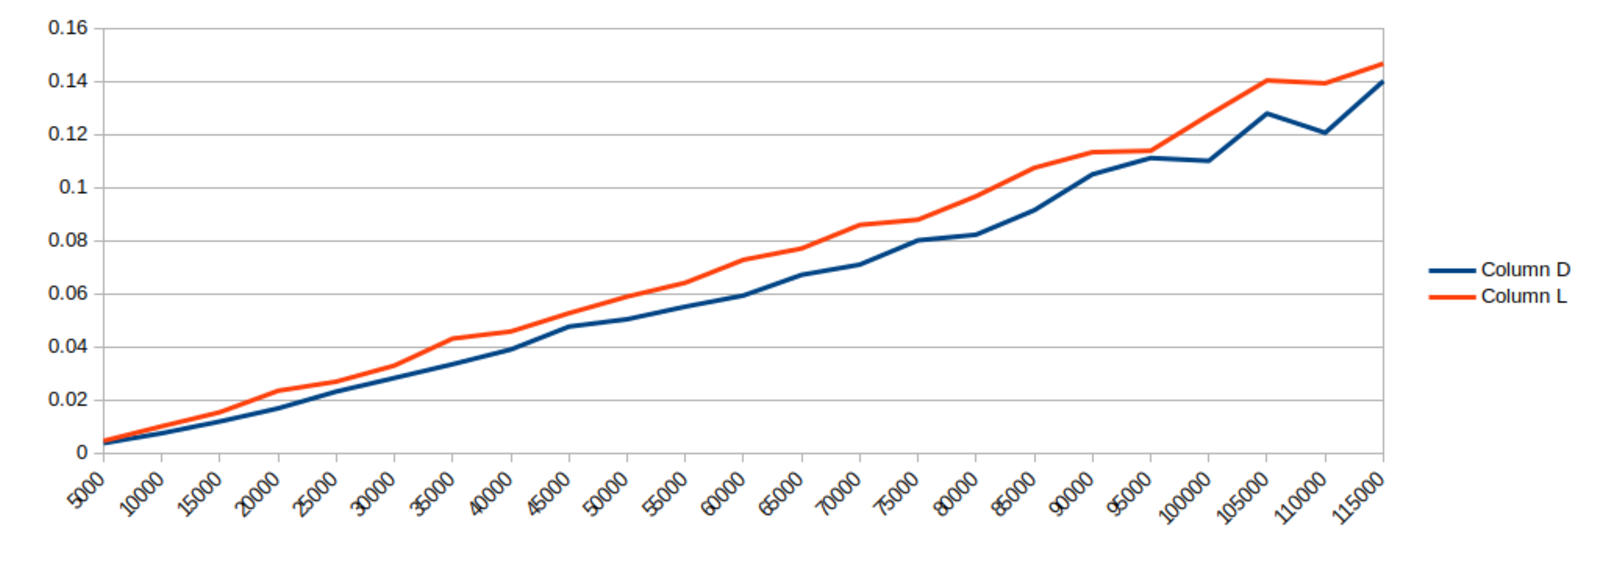
\includegraphics[left]{./images/running-time.eps}

This graph shows that the running time of the two algorithm is linear. This is further supported by the statistical analysis through linear regression. We have fit a line through the points with *figure out how to do this.*

\section{Analysing Datasets}

I will analyse three types of datasets. Two of the types are taken from real life data and one is synthetic. The first type is data that is the elevation of a mountain range in Canada. The second one is images. The third one is randomly generated graphs. The goal here is firstly to demonstrate where w-structures appear in the contour trees of real life data. The second goal is to analyse random graphs and derive statistical information on the probability of having large w-structures in contour trees of large data sets.


% @TODO Define the augmented and unaugmented controur tree
This table is for augmented contour trees.

\subsection{Mountain Range Data}

This is elevation data taken from the Canadian Mountains. Oh Canada is so great and amazing. Oh motherland of maple and Celine Dione I bow before you beautiful nature and spectacular mountains.

The datasets are all part of something. Explain where they are from.

% @TODO Add iterations needed for collapse 

\begin{center}
\begin{tabular}{l*{6}{c}r}
Dataset             & Vectices  & 2BFS  & DP    & NBFS  & Diameter  & Iterations\\
\hline
vanc                & 378       & 2     & 2     & 2     & 311       & -1 \\
vancouverNE         & 4851      & 4     & 5     & 5     & 1338      & -1 \\
vancouverNW         & 4900      & 5     & 5     & 5     & 1456      & -1 \\
vancouverSE         & 4950      & 6     & 6     & 6     & 1306      & -1 \\
vancouverSW         & 5000      & 4     & 4     & 4     & 1977      & -1 \\
vancouverSWNE       & 1250      & 5     & 5     & 5     & 423       & -1 \\
vancouverSWNW       & 1250      & 3     & 3     & 3     & 712       & -1 \\
vancouverSWSE       & 1275      & 3     & 3     & 3     & 759       & -1 \\
vancouverSWSW       & 1225      & 2     & 2     & 2     & 845       & -1 \\
icefield            & 57600     & 7     & 7     & 7     & 12280     & -1 \\
pukaskwa            & 180       & 180   & -1    & -1    & 374866    & -1 \\
gtopo30w020n40      & -1        & -1    & -1    & -1    & N/A       & -1 \\

\end{tabular}
\end{center}

All the vancouver data sets are similar. There we have a very low w-diameter compared to diameter. Speculate as to why that may be the case.

The most interesting case is pukaskwa. Notice how pukaskwa has 881600 edges this means that under logarithmic collapse we should take 13 iteration. Instead we do 90. This is a problem, no?

\subsection{Images}

*Find some images and test them and write about them.*

\subsection{Random Data}


Talk about the value of random data in providing statistics. It may not be realistic but we may draw conclusion about the distribution of w-diameters in random trees.

This is taken from generating random data sets and taking the distribution of the w-diameters of the trees. As you can see it kind of looks like a normal distribution. Interesting is it not? Talk about random samples and the law of large numbers.

Here the overall conclusion that can be obtained from this analysis.

\subsection{Conclusions}

These are the conclusions from the empirical study.

\begin{itemize}
    \item The w-diameter of a tree is a much better upper bound on the algorithm.
    \item The w-diameter can severely prevent logarithmic collapse.
    \item The w-diameter becomes prevalent in random samples of randomly generated tree. Therefore the law of large number will affect it.
\end{itemize}



Also find some data sets to analyse. Maybe do some medical 3-dimentional data sets.

Talk about why random data sets may not be completely reliable.

*Show some graphs and shit*

*Make some reflective summary of scheize*

\section{Finding the smallest W-structure}

An interesting question that arises is what is the smallest dataset that produces a w-structure of at least three kinks. This has educational value. It's also useful for out general understanding. It will also serve as a very important counterexample in the next chapter. It is good for counterexamples to be as small as possible. That way they it's easier to articulate the counterarguments.

\section{Getting the w-diameter from raw data}

This analysis was all well and good, but it doesn't do too much good as it is done after the contour tree has been computed. The next step is to produce and algorithm that either produces it from raw data or produces it from the join and split tree. The hope for this would that is there is some priori information before going into the merge phase of he algorithm, we may be able to avoid the serialisation along the kinky paths.

\section{Future work for the empirical study.}

Summarise things say what was successful, what was not. That kind of stuff.

This chapter does seem short. This is because most of the work put in the dissertation has either been theoretical which is in the previous chapters. or on impelmenting the newly created algorithms, which are in the appendix.

